\section{Electron densities}
\subsection{Electron density in the conduction band} \label{sec:electron_density}
For a 3D semiconductor the energy dispersion relation is:
\begin{equation}
	E(\vec{k}) = \frac{\hbar^2}{2m^*}(k^2_x + k^2_y + k^2_z) + E_{CB}(\vec{0})
\end{equation}
If we want the electron density at the conduction band, we can use the Fermi-Dirac distribution to know if a state is occupied and we will just sum over all possible $\vec{k}$ values.
\begin{equation}
	n = \frac{2}{V}\sum_{\vec{k}}^{}f(E(\vec{k})) \approx \frac{2}{V}\frac{V}{(2\pi)^3}\int d\vec{k} f(E(\vec{k})) \label{eqn:density}
\end{equation} \par
How can we make this approximation? \\
As we know from previous chapter, if the volume increases, the amount of k states in creases too which gives rise to a Riemann sum that becomes an integral. This is derived in short below:
\begin{align}
	\sum_{k_x} &= \dots \\
	&= \frac{1}{\Delta k_x}\sum_{k_x}\dots \Delta k_x \\
	\text{with }k_x = \frac{2\pi}{L_x}n_x \qquad &\approx \frac{1}{\Delta k_x}\int\dots dk_x \qquad \text{if }L_x \rightarrow \infty \\
	&= \frac{L_x}{2\pi}\int\dots dk_x
\end{align}
Can we work equation \ref{eqn:density} further out? If the integral is know, which it is, we can. As a sidenote, this integral can be written in spherical coordinates.
Furthermore, normally we work in the first BZ but now, we can without any trouble leave the boundaries at $-\infty$ and $\infty$. This is the case because the Fermi-Dirac distribution becomes 0 at $E = \infty$, see figure \ref{fig:fermidiracinenergyband}. Thus adding the Jacobian and filling in the boundaries gives:
\begin{align}
	n &\approx \frac{2}{V}\frac{V}{(2\pi)^3}\int_{-\infty}^{\infty} d\vec{k} f(E(\vec{k})) \\
	&= \frac{2}{(2\pi)^3}\int_{0}^{\infty}4\pi k^2 f(E(k)) dk
\end{align}
Working in energy might be easier than working in k-space. We use the following substitution:
\begin{align}
	dk &= \frac{dk}{dE}dE \\
	\frac{dE}{dk} &= \frac{d}{dk}(\frac{\hbar^2}{2m^*}k^2 + E_{CB}(\vec{0})) = \frac{\hbar^2 k}{m^*} \\
	k &= \sqrt{\frac{2m^*}{\hbar^2}(E-E_{CB}(\vec{0}))}
\end{align}
This then gives a final result for n:
\begin{align}
	n &= \frac{2}{(2\pi)^3}\int_{-E_{CB}(\vec{0})}^{\infty} 4\pi \frac{2m^*}{\hbar^2}(E-E_{CB}(\vec{0})) f(E(\vec{k})) \frac{m^*}{\hbar^2} \frac{1}{\sqrt{\frac{2m^*}{\hbar^2}(E-E_{CB}(\vec{0}))}} dE\\
	&= \frac{2}{(2\pi)^3} 4\pi \frac{m^*}{\hbar^2} \int_{-E_{CB}(\vec{0})}^{\infty} \sqrt{\frac{2m^*}{\hbar^2}(E-E_{CB}(\vec{0}))} f(E(\vec{k})) dE \\
	&= \frac{(2m^*)^{3/2}}{2\pi^2\hbar^2} \int_{-E_{CB}(\vec{0})}^{\infty} \sqrt{(E-E_{CB}(\vec{0}))} f(E(\vec{k})) dE \label{eqn:dinsity_}
\end{align}

\subsubsection{Simplifying the electrons density $n$}
Now, working this integral out even further is difficult. But we can use the well known Fermi-Dirac integral of order 1/2. The Fermi-Dirac integrals is:
\begin{equation}
	F_{1/2}(\xi) = \frac{2}{\sqrt{\pi}}\int_{E_{CB}(\vec{0})}^{\infty} \frac{x^{1/2}}{1 + e^{x-\xi}} dx
\end{equation}
If we use the substitute $\xi = \frac{\mu - E_{CB}(\vec{0})}{kT}$ we get:
\begin{align}
	n &= 2 \left(\frac{m^*kT}{2\pi\hbar^2}\right)^{3/2} F_{1/2}\left(\frac{\mu - E_{CB}(\vec{0})}{k_BT}\right) \\
	&\qquad \text{with } N_C = 2 \left(\frac{m^*kT}{2\pi\hbar^2}\right)^{3/2}
\end{align}
$N_C$ is the effective density of states. \\ \par
Now, as we know, if $\mu$ is sufficiently far away from $E_{CB}(\vec{0})$ (meaning $E_{CB}(\vec{0}) - \mu > 4k_BT$), then the Fermi-Dirac distribution can be approximated by the Maxwell-Boltzmann distribution. This results in:
\begin{align}
	n &\approx \frac{(2m^*)^{3/2}}{2\pi^2\hbar^3} \int_{E_{CB}(\vec{0})}^{\infty} (E-E_{CB}(\vec{0}))^{1/2} e^{-\frac{1}{k_BT}(E-\mu)} dE \\
	\text{take } x = \frac{E-E_{CB}(\vec{0})}{k_BT} \qquad &= \frac{(2m^*)^{3/2}}{2\pi^2\hbar^3} \sqrt{k_BT} \int_{E_{CB}(\vec{0})}^{\infty} \left(\frac{E-E_{CB}(\vec{0})}{k_BT}\right)^{1/2} e^{-\frac{1}{k_BT}(E-\mu)} dE \\
	&= \frac{(2m^*)^{3/2}}{2\pi^2\hbar^3} \sqrt{k_BT} e^{-\frac{E_{CB}(\vec{0})-\mu}{k_BT}} \int_{0}^{\infty} x^{1/2} e^{-x} dx k_BT \\
	&= \frac{(2m^*)^{3/2}}{2\pi^2\hbar^3} (k_BT)^{3/2} e^{-\frac{E_{CB}(\vec{0})-\mu}{k_BT}} \int_{0}^{\infty} x^{1/2} e^{-x} dx \label{eqn:knownitegral}
\end{align}
The integral in equation \ref{eqn:knownitegral} is a well known Gaussian integral and can be easily calulated to obtain a value of $\frac{\sqrt{\pi}}{2}$. Meaning the final expression for n is:
\begin{equation}
	n \approx \frac{(2m^*)^{3/2}}{2\pi^2\hbar^3} (k_BT)^{3/2} e^{-\frac{E_{CB}(\vec{0})-\mu}{k_BT}} \frac{\sqrt{\pi}}{2} = N_C e^{-\frac{E_{CB}(\vec{0})-\mu}{k_BT}}
\end{equation}
This approximation is true for $E_{CB}(\vec{0}) - \mu > 4k_BT$ which are mostly non-degenerate semiconductors.

\subsection{Hole density in the valence band}\label{sec:holes}
We will derive the hole densities for both heavy and ligh holes. The according dispersion relations are:
\begin{align}
	E_{hh} &= -\frac{\hbar^2k^2}{2m_{hh}^*} \qquad \text{with } m^*_{hh} = -m_1^* > 0 \\
	E_{lh} &= -\frac{\hbar^2k^2}{2m_{lh}^*} \qquad \text{with } m^*_{lh} = -m_2^* > 0
\end{align}
Then
\begin{align}
	m_{hh}^* &= -\left\left[\frac{1}{\hbar^2}\frac{\delta^2 E_{hh}}{\delta k_i^2}\right]^{-1}\right|_{\vec{k} = \vec{0}} > 0 \\
	m_{lh}^* &= -\left\left[\frac{1}{\hbar^2}\frac{\delta^2 E_{lh}}{\delta k_i^2}\right]^{-1}\right|_{\vec{k} = \vec{0}} > 0
\end{align}
We immediatly see what we mean with heavy and light holes. Because the effective mass is inverse proportional to the second derivative of the energy, we see that $m_{hh}^* > m_{lh}^*$ for every energy. The according bands can be seen in figure \ref{fig:heavyandlight_holes}.
\begin{figure}
	\centering
	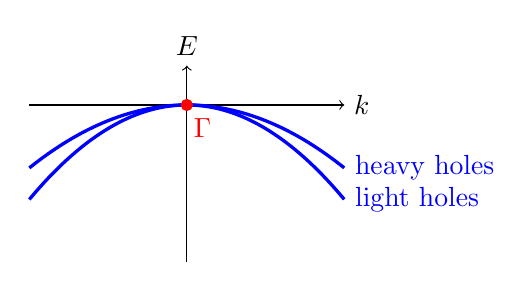
\begin{tikzpicture}[domain=-2:2]
		\draw[->, black]	(-2, 0) to (2, 0) node[right]{$k$};
		\draw[->, black]	(0, -2) to (0, 0.5) node[above]{$E$};

		\draw[blue, very thick] plot[samples=200] (\x, -0.3*\x*\x) node[right]{light holes};
		\draw[blue, very thick] plot[samples=200] (\x, -0.2*\x*\x) node[right]{heavy holes};

		\filldraw[red] 		(0, 0) circle (2pt);
		\draw[red]			(0.2, -0.05) node[below]{$\Gamma$};
	\end{tikzpicture}
	\caption{Graphical meaning of heavy and light holes in the conduction band}
	\label{fig:heavyandlight_holes}
\end{figure}
\subsubsection{What is a hole?}
As we know at $T = 0K$, the conduction band is empty and the valence band is completely filled. But at a temperature $5 > 0K$, there is a chance that the valence band misses an electron. This chance only gets higher when getting closer to $\mu$. Then the Fermi-Dirac distribution can be defined for the abscence of electrons:
\begin{equation}
	1 - f(E) = \frac{1}{1 + e^{\beta(\mu - E)}} = f_h(E) \label{eqn:hole_fermi-dirac}
\end{equation}
This will be defined as the Fermi-Dirac distribution of holes, which in their turn are defined by the abscence of an electron. Holes can also be treated as quasi-particles (section \ref{sec:quasi_particles}). \nt{Note the change of the signs in equation \ref{eqn:hole_fermi-dirac} compared to equation \ref{eqn:elec_fermi-dirac}}

\subsubsection{Calculation of the hole density}
This part will be practically the same as section\ref{sec:electron_density}, therefore only the differences will be highlighted.
Again, we start with:
\begin{align}
	p &= \frac{2}{V}\sum_{\vec{k}}^{}f(E_{\alpha}(\vec{k})) \qquad \text{with } \alpha = hh,\, lh \\
	E_{\alpha}(\vec{k}) &= -\frac{\hbar^2}{2m_{\alpha}^*}k^2 \\
\end{align}
This results in:
\begin{align}
	p &= N_V F_{1/2}\left(\frac{E_{VB}(\vec{0}) - \mu}{k_BT}\right) \\
	N_V &= 2\left(\frac{m_{d,h}^*k_BT}{2\pi\hbar^2}\right)^{3/2} \label{eqn:n_v} \\
	m_{d,h}^* &= \left[(m_{hh}^*)^{3/2} + (m_{lh}^*)^{3/2}\right]^{2/3}
\end{align}
With $m_{d,h}^*$ the density of states effective mass for holes. Because we worded with two valence bands, we get this somewhat more complex definition for the effective mass. If there is only one valence band the equation simlifies to $m_h^*$. Notice that there are many similarities between these equation and the ones for electrons.

\subsubsection{Simplifying the hole density}
For this we can use the following rule: if $ \mu -E_{VB}(\vec{0}) > 4k_BT $ we can use the Maxwell-Boltzmann relation. This result in the following equation for the hole density:
\begin{equation}
	p = N_Ve^{-\frac{E_{VB}(\vec{0}) - \mu}{k_BT}}
\end{equation}

\ex{Try at home}{
	When using equation \ref{eqn:n_v}, we can show that $p_{lh} < p_{hh}$. Use the following equation to separate equation \ref{eqn:n_v}:
	\begin{equation*}
		p &= p_{hh} + p_{lh} \\
	\end{equation*}
	Why can we show this? \\
	\textbf{Solution: \quad because \begin{equation} \frac{p_{lh}}{p_{hh}} = \frac{N_{V, lh}}{N_{V, hh}} = \left(\frac{m_{lh}^*}{m_{hh}^*}\right)^{3/2} \end{equation} where \begin{equation} \frac{m_{lh}^*}{m_{hh}^*} < 0 \end{equation} }
}

\subsection{An example}
\ex{Try at home - Si}{
	When calculating the electron density for the conduction band for silicon one gets the following:
	\begin{align}
		E_{\alpha}(\vec{k}) &= E_{CB}(\vec{0}) + \frac{\hbar^2}{2}\left[\frac{(k_x - k_{0, \alpha, x})^2}{m^*_l} + \frac{(k_y - k_{0, \alpha, y})^2}{m^*_t} + \frac{(k_z - k_{0, \alpha, z})^2}{m^*_t}\right] \\
		n &= \frac{2}{V} \sum_{\vec{k}, \alpha}^{}f(E_{\alpha}(\vec{k})) \\
		&= N_C F_{1/2}(\frac{\mu - E_{CB}(\vec{0})}{k_BT}) \\
		N_C &= 2\left(\frac{m_{d,e}^*k_BT}{2\pi\hbar^2}\right)^{3/2} \\
		m_{d,e}^* &= (K^2m_l^*^2m_t^*)
	\end{align}
	With $\alpha$ between $1$ and $6$, and $K$ the amount of conduction band minima.\\
	To get to the solution, perform a coordinate transformation which scales the k values according to the relative effective masses.
}

\section{Law of mass action}
Suppose we restrict ourselves to non-degenerate semiconductors, meaning we can use the Maxwell-Bolzmann equations, and we take the following product:
\begin{equation}
	np = N_CN_Ve^{\frac{E_v-E_c}{k_BT}} = N_CN_Ve^{-\frac{E_g}{k_BT}}
\end{equation}
Thus we can conclude that the product $np$ depends on:
\begin{itemize}
	\setlength\itemsep{0pt}
	\item $T$
	\item $N_C$, $N_V$; but not $\mu$
	\item $E_g$
\end{itemize}
For intrinsic semiconductors we will say that
\begin{equation}
	np = n_i^2
\end{equation}
Here, $n_i$ is the intrinsic concentration of the semiconductor. Moreover $n \approx p = n_i$.
\nt{This is only valid when using Maxwell-Boltzmann!}

\section{Determining the chemical potential $\mu$}
Say we have $N = $ the total amount of electrons and we have the following band diagrams for $T = 0K$ and $T > 0K$:
\begin{figure}
	\centering
	\begin{tikzpicture}

	\end{tikzpicture}
	\caption{Simple qualitative band diagrams}
	\label{fig:determining_mu}
\end{figure}
We know that the total density $n_{tot}$ is conserved
\begin{equation}
	\frac{N}{V} = n_(tot) \quad \Rightarrow \quad n = p
\end{equation}
Because every hole is generated by an electron, and we know no electron is annihilated, we can say that (when using Maxwell-Boltzmann approximations):
\begin{align}
	&N_Ce^{-\frac{E_c - \mu}{k_BT}} = N_Ve^{-\frac{\mu - E_v}{k_BT}} \\
	\iff\quad&\mu = \frac{k_BT}{2}\left[\ln\frac{N_V}{N_C} + \frac{E_v + E_c}{k_BT}\right] = \mu(T) \\
	\iff\quad&\mu(T) = \frac{E_v + E_c}{2} + \frac{k_BT}{2}\ln\frac{N_V}{N_C}
\end{align}
We have a temperature dependance for $\mu$ meaning that we get two cases:
\begin{enumerate}
	\item $T = 0K$: $\mu(T = 0) = E_v + \frac{E_g}{2} = E_i$; \qquad  where $E_i$ is called the intrinsic energy band.
	\item $T > 0K$: $\mu(T) = \mu(0) + \frac{k_BT}{2}\ln\frac{N_V}{N_C} = \mu(0) + \Delta\mu(T)$; \qquad where, yet again, we have two possabilities:
	\begin{enumerate}
		\setlength\itemsep{0pt}
		\item $\Delta\mu(T) > 0$ if $N_v > N_c$
		\item $\Delta\mu(T) < 0$ if $N_v < N_c$
	\end{enumerate}
\end{enumerate}
We can say that $\mu$ will shift towards the band with the lowest effective density states. Yet, this shift is very small, i.e., for Si the $\Delta\mu(T)$ is of the order of $1meV$.
\nt{For Si at room temperature $n = p = n_i \approx 10^{10} cm-{3}$.}
